\newpage

\begin{problem}
  Sketch the graph of the function
  \begin{equation*}
    \sum_{k=0}^n\|l_k(x)\|, a \leq x \leq b
  \end{equation*}
  Consider the problem of placing the interpolation points ${x_0,
  \dots, x_n }$ in a way that minimizes $\|X\|$. Show that it is
  suitable to let $x_0$ and $x_n$ have the values $a$ and $b$
  respectively. Investigate the position(s) of the other point(s) when
  $n = 2$ and $n = 3$.
\end{problem}
0
%--------------------------------------------------------------------%

\begin{solution}
  \begin{enumerate}
  \item[{\bf end points}] In figure~\ref{fig:3} we see at the ends of
    the interval after the out-most Chebyshev point all polynomials
    start to diverge away from zero. Therefore
    $\sum_{k=0}^n|l_k(x)|$ will increase rapidly towards the end
    of the interval. Figure~\ref{fig:4edge} illustrates this
    behavior. This result suggests that it is preferable to place
    $x_0$ and $x_n$ at the end points of the interval or at least
    very close.

    \begin{figure}[!ht]
      \centering 
      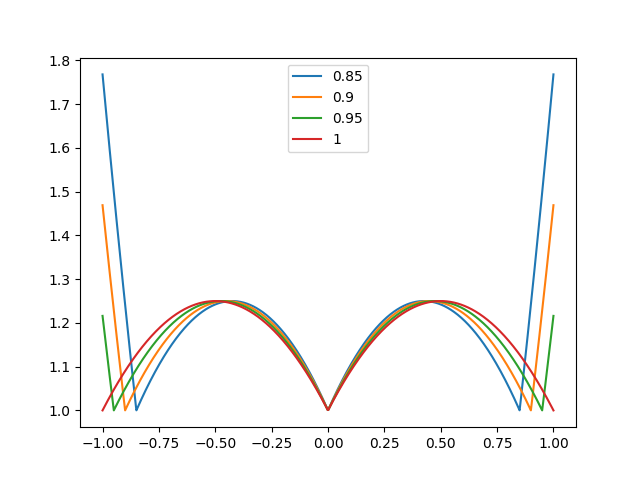
\includegraphics[scale = 0.5]{code/task_4_edge.png}
      \caption{Plot of $\sum_{k=0}^n|l_k(x)|$ with three points. $\{-x,
        0, x\}$ for $x \in \{0.85, 0.9, 0.95, 1\}$}
      \label{fig:4edge}
    \end{figure}

  \item[{\bf case: $n=2$}] In the case of three points it is clear from figure
    \ref{fig:4n2} that $x_1=0$ for minimized norm of the operator. Any
    deviation from that position will increase one of the two local
    maxima but when $x_1=0$ the two maxima are equal.
    \begin{figure}[!ht]
      \centering 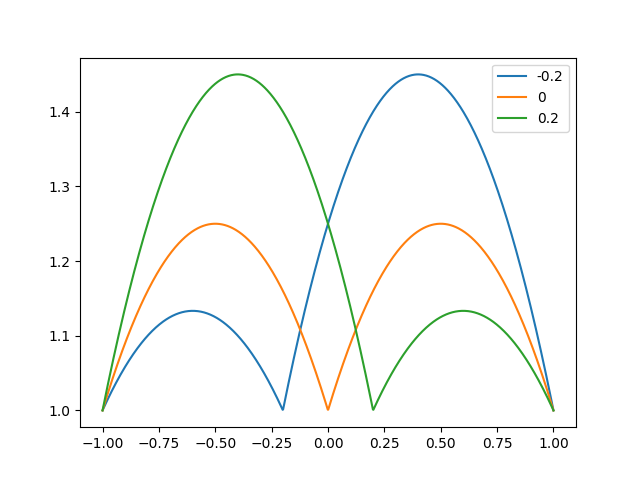
\includegraphics[scale = 0.5]{code/task_4_n2.png}
      \caption{Plot of $\sum_{k=0}^n|l_k(x)|$ with three points. $\{-1,
        x, 1\}$ for $x \in \{-0.2, 0, 0.2\}$}
      \label{fig:4n2}
    \end{figure}

  \item[{\bf case: $n=3$}] With four points the pattern in figure \ref{fig:4n3} is clear. Reducing the distance between two points
    reduce the maximum between. The cost however will be that another
    distance will increase and thus increase that corresponding
    maxima. The minimal value is obtained when all the local maxima is
    the    equal. From figure\ref{fig:4n3} we see that this point is
    somewhere between $-x_1 = x_2 = 0.4$ and $0.5$. 
    \begin{figure}[!ht]
      \centering
      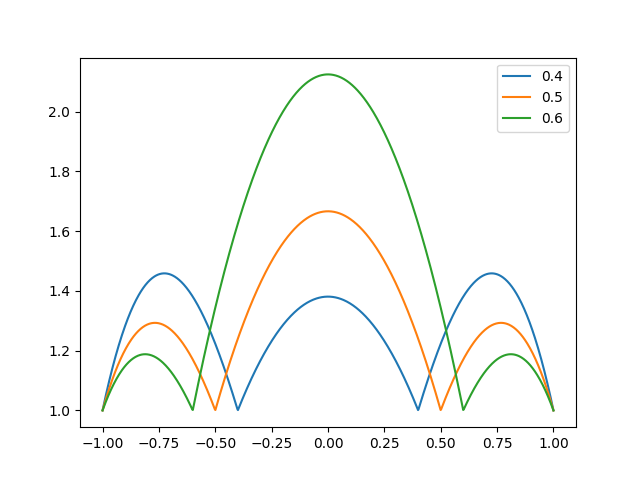
\includegraphics[scale = 0.5]{code/task_4_n3.png}
      \caption{Plot of $\sum_{k=0}^n|l_k(x)|$ with four
        points. $\{-1, -x, 0, x, 1\}$ for $x \in \{0.4, 0.5, 0.6\}$}
      \label{fig:4n3}
    \end{figure}
  \end{enumerate}
\end{solution}

%%% Local Variables:
%%% TeX-master: "report.tex"
%%% End:
